\subsubsection{Vision}
\label{sec:Kap-6.1.2.1}

Im Rahmen des Requirements Engineering ist eine Produktvision (kurz: Vision, synonym: Systemidee) eine oft noch recht unkonkret formulierte Darstellung des Zustands, der mit dem Einsatz des Softwareprodukts erreicht werden soll. Die Vision soll vor allem deutlich machen, \textbf{warum} das Softwareentwicklungsprojekt (bzw. der Kauf einer Software) gestartet wird und inwiefern dadurch die aktuelle Situation verbessert wird. Im Einzelnen gehören zu einer Vision:

\begin{itemize}
	\item \textbf{\sttpHervorhebung{Die Darstellung der Ausgangslage und der Motivation für die 
			\linebreak %%% für Druck
			Projektdurchführung}}: Die Darstellung beinhaltet die Beschreibung der aktuellen Situation inklusiver bekannter Probleme (vor Einsatz des Produkts) und Erwartungen -- manchmal auch nur Hoffnungen --, inwiefern die \mbox{Situation} verbessert wird, wenn das Softwareprodukt eingesetzt wird. Hier geht es darum, den positiven Einfluss des einzuführenden Produkts in Bezug auf über\-geordnete Unternehmensziele, Arbeitsabläufe und das existierende Unter-
			\linebreak %%% für Druck
			nehmensumfeld zu skizzieren. 
	\item \textbf{\sttpHervorhebung{Eine skizzenhafte Beschreibung der Hauptcharakteristika des Softwareprodukts}}: Auf einem sehr hohen Abstraktionslevel werden die wichtigsten geplanten Eigenschaften und Funktionalitäten des Softwareprodukts beschrieben. Dazu können auch Einschränkungen gehören, welche Aufgaben\-bereiche nicht von der Software übernommen werden sollen (\zb wenn im Zoobeispiel die Verwaltung der Tierarztrechnungen nicht Bestandteil der \mbox{neuen} Zoo-Software sein sollte).
	\item \textbf{\sttpHervorhebung{Ein grober Überblick über Verbindungen zu anderen Systemen}}: Es sollte dargestellt werden, in welcher Umgebung das neue Softwareprodukt eingesetzt wird. Zu dieser Umgebung gehören andere im Unternehmen eingesetzte Softwareprodukte, zu denen zukünftig Schnittstellen existieren sollen. Es geht aber auch um die Einbindung des Softwareprodukts in existierende Geschäfts\-prozesse und um die Verbindungen zwischen dem neuen Produkt und der existierenden oder neu zu schaffenden Hardwareumgebung.
\end{itemize}

Aus der Vision werden durch Konkretisierung und Ausdifferenzierung der genannten Aspekte die Ziele des Softwareeinsatzes sowie Produktumfang und Systemkontext abgeleitet. Die Beschreibung der Hauptcharakteristika bildet zudem die Basis für die Spezifizierung der wichtigsten Komponenten des zukünftigen Produkts.

Visionen von Softwareprodukten können unterschiedliche Schwerpunkte setzen. Insbesondere im agilen Umfeld steht oft der Aspekt der Motivation im Vordergrund der Vision, während die Beschreibung der Hauptcharakteristika weniger Aufmerksamkeit bekommt. Bei Softwareentwicklungsprojekten, deren Inhalt die Ablösung eines existierenden Produkts durch eine neue Version bzw. ein neueres Produkt derselben Art ist, ergeben sich die gewünschten Charakteristika des neuen Produkts häufig aus den Problemen mit dem alten Produkt. In solchen Fällen findet man eher eine sehr knappe Beschreibung der Motivationslage und dafür schon recht konkrete Beschreibungen der Hauptcharakteristika.

Eine Vision kann unterschiedlich umfangreich sein, zum Beispiel auch nur wenige Sätze umfassen. In der Regel bewegt sich der Rahmen zwischen einer halben Seite und maximal zwei Seiten Umfang, \marginline{Formen von Visionen} wobei es sich nicht zwingend um klassische Textdokumente handeln muss. So kann auch über eine Kombination aus Stichpunkten und Grafiken am Whiteboard eine Vision kommuniziert werden. \cite[43 \psqq]{oes13} schlägt vor, für die Vision einen Produktkarton zu gestalten, wie man ihn als Verpackung eines realen (gegenständlichen) Produkts kennt. Auf diese Weise wird die Produktvision für alle Projektbeteiligten auch plastisch sichtbar. Gleichzeitig beschränkt der Produktkarton den Umfang der Vision und erfordert es, sie geeignet zu strukturieren, da man sich überlegen muss, welche Informationen auf welcher Seite des Kartons platziert werden sollen. Eine solche plastische Kommunikation der Vision ist auch im agilen Umfeld -- unter dem englischen Begriff vision boxing -- bekannt.

Der \marginline{abweichende Definitionen} Begriff Vision gehört zu den Begriffen im Softwareengineering, zu denen Sie von vier Autoren und Autorinnen vier verschiedene Definitionen erhalten. Ein sehr grundsätzlicher Unterschied besteht in der Beantwortung der Frage, ob Rahmenbedingungen und Restriktionen, wie die angesetzten Zeit- und Kostenbudgets für das Softwareentwicklungsprojekt oder vorgegebene Hardwareumgebungen für das zukünftige Softwareprodukt, Bestandteil der Vision sein sollten. Hier gilt für dieses Modul: Sie sind dann Bestandteil der Vision, wenn sie direkt das Softwareprodukt betreffen (\zb was soll das Softwareprodukt nicht tun; welche Qualitätsstandards sind einzuhalten) oder wenn sie sich auf die Umgebung beziehen, in der das Softwareprodukt eingesetzt werden soll (\zb welche Geschäftsprozesse dürfen nicht verändert werden; welche Einschränkungen existieren durch vorhandene Hardwarekomponenten). Rahmenbedingungen, die sich auf das Softwareentwicklungs\textbf{projekt} beziehen (\zb das Budget oder die Restriktion, dass der Softwarearchitekt dem Projekt nur zwei Tage pro Woche zur Verfügung steht) sind nicht Bestandteil der Vision. Sehr wohl aber müssen Vision und projektbezogene Rahmenbedingungen in Einklang gebracht werden, wenn das Projekt erfolgreich verlaufen soll. 

Ein weiterer Diskussionspunkt im Kontext des Vision-Begriffs ist, ob die Ziele des Einsatzes des Softwareprodukts ebenfalls Bestandteil der Vision sind. Aufmerksamen Leserinnen und Lesern dürfte nicht entgangen sein, dass unsere Antwort auf diese Frage \textbf{Nein} lautet: 

\begin{itemize}[
	label={\sttpHervorhebung{$\Rightarrow$}},
	]
	\item Die Vision ist die Basis, aus der (unter anderem) die Ziele abgeleitet werden. Vision und Ziele bewegen sich somit auf unterschiedlichen Abstraktions\-niveaus.
\end{itemize}

Abbildung~\ref{fig:von_vision_zu_anforderungen} zeigt eine Erweiterung der Abbildung~\ref{fig:stakeholder_ziele_produktumfang_anfoderungen} aus Abschnitt~\ref{sec:Kap-6.1}. Ergänzt ist hier zum einen der Begriff der Vision und sein Zusammenhang zu Zielen und Produktumfang. Zum anderen ist der Begriff des Systemkontexts hinzugekommen, mit dem wir uns in Abschnitt~\ref{sec:Kap-6.1.3} näher beschäftigen werden. 

\vspace{\baselineskip} %%% für Druck
\vspace{\baselineskip} %%% für Druck

\begin{figure}[h!]
	%\centering
	\begin{addmargin*}[0cm]{-\marginparwidth}
	\begin{addmargin*}[0cm]{-\marginparsep}
		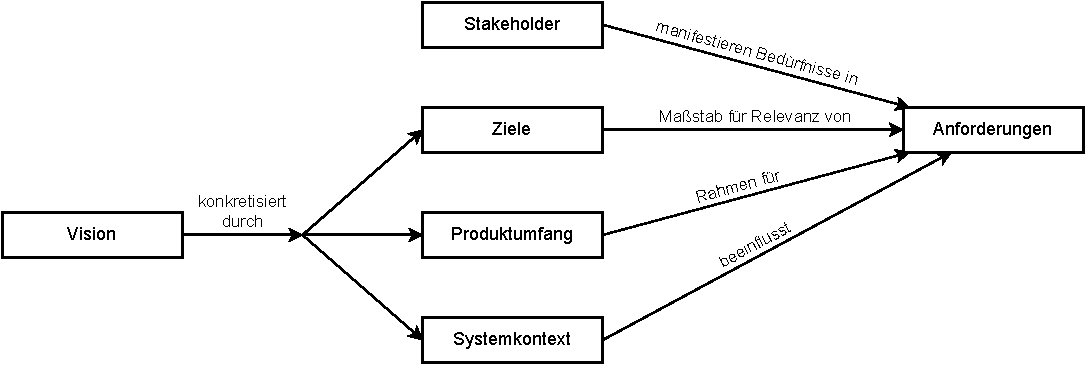
\includegraphics[scale=0.95]{Bilder/Kapitel-6/begriffe-version2.pdf}
		\caption{Von der Vision zu den Anforderungen}
		\label{fig:von_vision_zu_anforderungen}
	\end{addmargin*}
	\end{addmargin*}
\end{figure}

\pagebreak %%% für Druck

Wir \marginline{Sinn der Vision} möchten das Thema Vision mit der grundsätzlichen Frage abschließen: Wozu braucht man eine übergeordnete Vision, warum beginnt man nicht direkt mit der Formulierung von Zielen und Produktumfang?

\begin{itemize}[
	label={\sttpHervorhebung{$\Rightarrow$}},
	]
	\item Die Vision ist nötig, um die Produktziele, den Produktumfang und auch die Bedürfnisse der einzelnen Stakeholder des Projekts auf die übergreifenden Ziele, die aktuelle Situation und die Zukunftspläne des Unternehmens zu fokussieren. Wir erinnern daran, dass die Ziele der Maßstab für die Relevanz der Anforderungen sind. Der Maßstab für die Relevanz der einzelnen Ziele wiederum ist die Vision. Ähnliches gilt für den Produktumfang: Der Produktumfang ist der Rahmen, in den die Anforderungen passen müssen. Der Rahmen, in den der Produktumfang passen muss, ist die Vision. 
\end{itemize}